% !TeX root = ../main.tex
% Add the above to each chapter to make compiling the PDF easier in some editors.

\chapter{Evaluation}\label{chapter:evaluation}
We now turn to the evaluation of the streaming protocols we presented, referred to in this chapter as deprioritize B-frames and skip old \acp{GoP}. We begin by describing the testbed and metrics used to measure the performance of our streaming protocols. Then, we present the results collected from multiple test runs of our approaches across different network profiles. We conclude with a qualitative evaluation, in which we discuss additional factors that should be accounted for when considering either approach.

\section{Testbed}
Our testbed emulates network bandwidth limits during a live streaming session between the client and the origin server. We perform multiple test runs for each streaming protocol, in which we first launch the client, establish a connection to the server, and subscribe to the video stream. Once playback starts, we simulate various types of network patterns that are representative of real-world network conditions and collect relevant metrics. The network profiles used, which are taken from Twitch's 2020 Grand Challenge on low-latency live streaming \parencite{twitchGrandChallengeAdaptation}, are shown in \autoref{fig:bandwidth_profiles}.

\begin{figure}
    \centering
    
    % First row - Cascade profiles
    \begin{subfigure}[b]{0.3\textwidth}
        \centering
        \begin{tikzpicture}
            \begin{axis}[
                width=\textwidth,
                % xlabel={Time (s)},
                % ylabel={Bandwidth (Kbit/s)},
                ymin=0, ymax=1300, ytick distance=200,
                ymajorgrids=true,
                grid style=dashed,
                tick label style={font=\footnotesize},
                label style={font=\footnotesize},
            ]
            \addplot[red, const plot, thick, solid, mark=*] coordinates {
                (0,1200) (30,1200) (30,800) (60,800) (60,400) (90,400)
                (90,800) (120,800) (120,1200) (150,1200)
            };
            \end{axis}
        \end{tikzpicture}
        \caption{\footnotesize CASCADE}
    \end{subfigure}
    \begin{subfigure}[b]{0.3\textwidth}
        \centering
        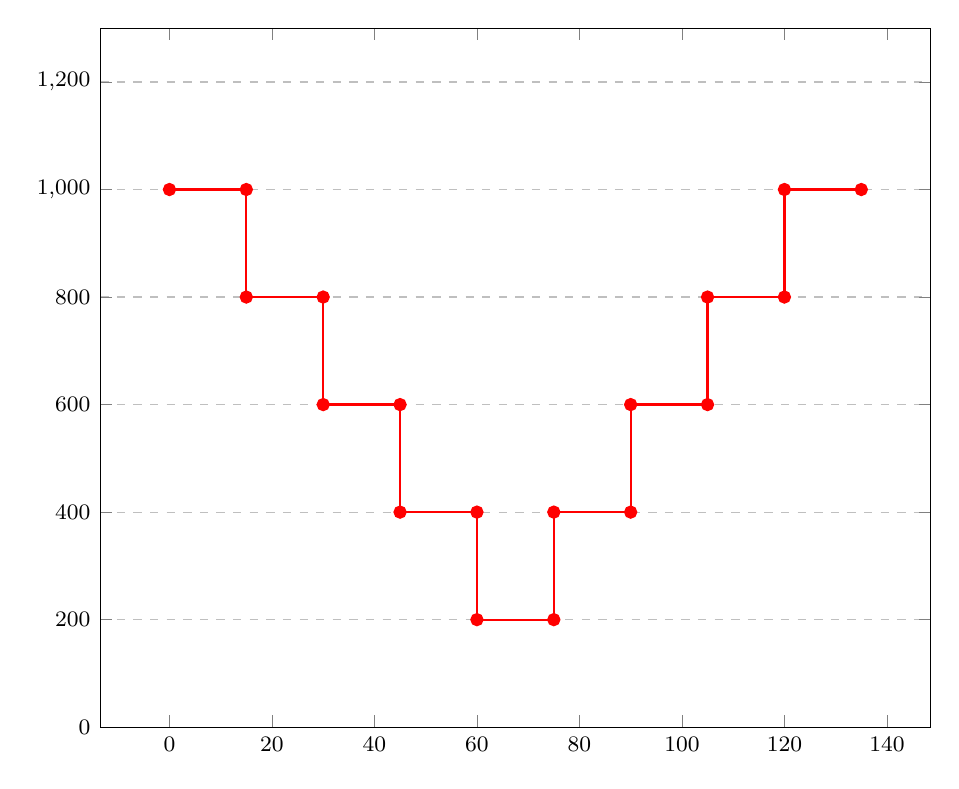
\begin{tikzpicture}
            \begin{axis}[
                width=\textwidth,
                % xlabel={Time (s)},
                % ylabel={Bandwidth (Kbit/s)},
                ymin=0, ymax=1300, ytick distance=200,
                ymajorgrids=true,
                grid style=dashed,
                tick label style={font=\footnotesize},
                label style={font=\footnotesize},
            ]
            \addplot[red, const plot, thick, solid, mark=*] coordinates {
                (0,1000) (15,1000) (15,800) (30,800) (30,600) (45,600) (45,400) (60,400)
                (60,200) (75,200) (75,400) (90,400) (90,600) (105,600) (105,800) (120,800)
                (120,1000) (135,1000)
            };
            \end{axis}
        \end{tikzpicture}
        \caption{\footnotesize INTRA\_CASCADE}
    \end{subfigure} 

    \vspace{1em}
    
    % Second row - Other profiles
    \begin{subfigure}[b]{0.3\textwidth}
        \centering
        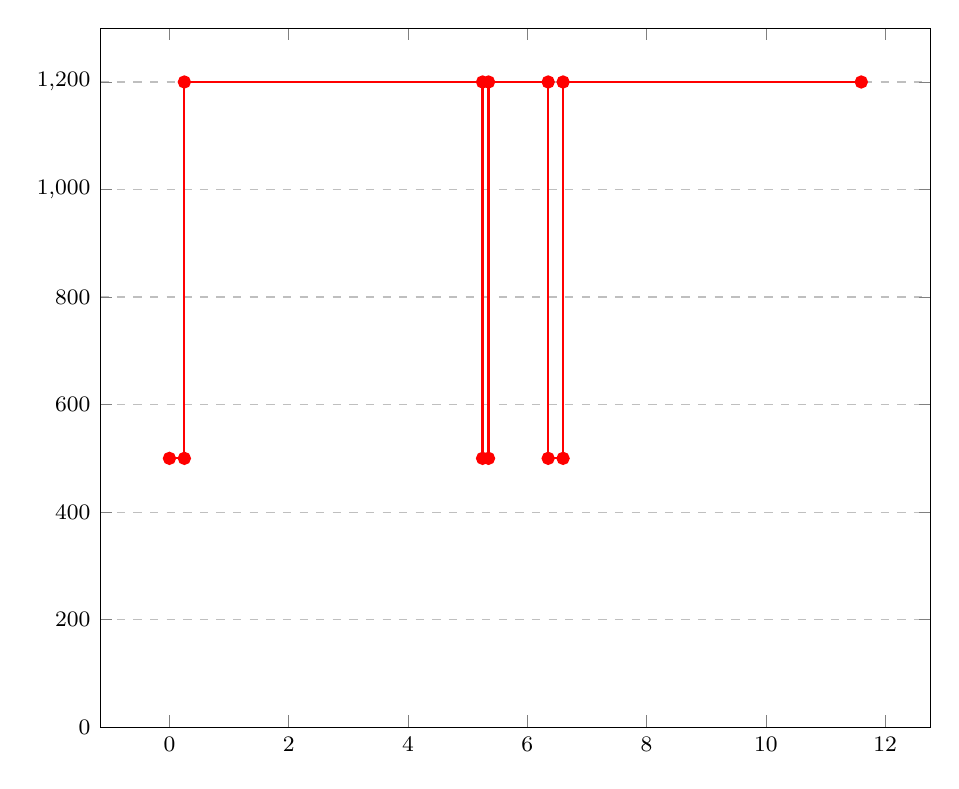
\begin{tikzpicture}
            \begin{axis}[
                width=\textwidth,
                % xlabel={Time (s)},
                % ylabel={Bandwidth (Kbit/s)},
                ymin=0, ymax=1300, ytick distance=200,
                ymajorgrids=true,
                grid style=dashed,
                tick label style={font=\footnotesize},
                label style={font=\footnotesize},
            ]
            \addplot[red, const plot, thick, solid, mark=*] coordinates {
                (0,500) (0.25,500) (0.25,1200) (5.25,1200) (5.25,500) (5.35,500)
                (5.35,1200) (6.35,1200) (6.35,500) (6.6,500) (6.6,1200) (11.6,1200)
            };
            \end{axis}
        \end{tikzpicture}
        \caption{\footnotesize FAST\_JITTERS}
    \end{subfigure}
    \begin{subfigure}[b]{0.3\textwidth}
        \centering
        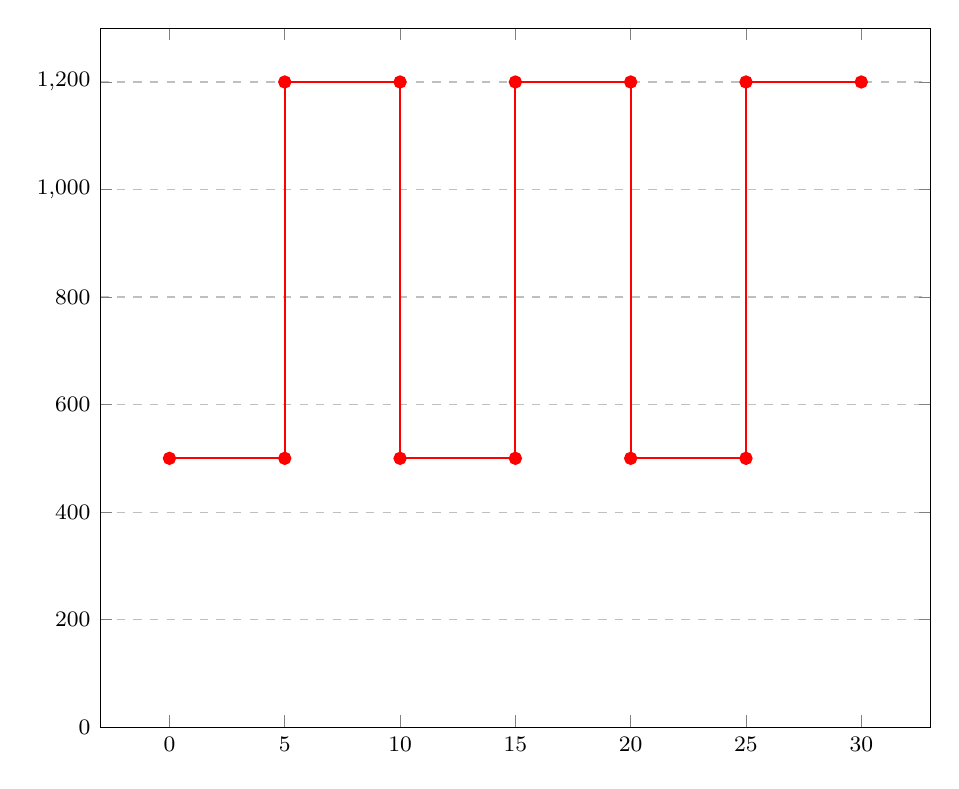
\begin{tikzpicture}
            \begin{axis}[
                width=\textwidth,
                % xlabel={Time (s)},
                % ylabel={Bandwidth (Kbit/s)},
                ymin=0, ymax=1300, ytick distance=200,
                ymajorgrids=true,
                grid style=dashed,
                tick label style={font=\footnotesize},
                label style={font=\footnotesize},
            ]
            \addplot[red, const plot, thick, solid, mark=*] coordinates {
                (0,500) (5,500) (5,1200) (10,1200) (10,500) (15,500) (15,1200) (20,1200)
                (20,500) (25,500) (25,1200) (30,1200)
            };
            \end{axis}
        \end{tikzpicture}
        \caption{\footnotesize SLOW\_JITTERS}
    \end{subfigure}
    \begin{subfigure}[b]{0.3\textwidth}
        \centering
        \begin{tikzpicture}
            \begin{axis}[
                width=\textwidth,
                % xlabel={Time (s)},
                % ylabel={Bandwidth (Kbit/s)},
                ymin=0, ymax=1300, ytick distance=200,
                ymajorgrids=true,
                grid style=dashed,
                tick label style={font=\footnotesize},
                label style={font=\footnotesize},
            ]
            \addplot[red, const plot, thick, solid, mark=*] coordinates {
                (0,1200) (10,1200) (10,300) (20,300) (20,800) (30,800)
            };
            \end{axis}
        \end{tikzpicture}
        \caption{\footnotesize SPIKE}
    \end{subfigure}

    \vspace{1em}

    \caption{Bandwidth profiles - Bandwidth (Kbit/s) vs. time (s)}
    \label{fig:bandwidth_profiles}
\end{figure}

We use dummynet\footnote{\url{https://man.freebsd.org/cgi/man.cgi?dummynet}} to emulate a link with limited bandwidth between the origin server and the client. Dummynet is a traffic shaping tool that simulates queue size and bandwidth limitations, delays, and packet loss by intercepting traffic between the transport protocol layers \parencite{rizzoDummynetSimpleApproach1997}. % TODO: I can expand on how it works if i want
In order to simulate the bandwidth limits, we use a dummynet \textit{pipe} and feed traffic from the client to the server and vice versa into the pipe using PF\footnote{\url{https://www.openbsd.org/faq/pf/}} (Packet Filter).

The client and origin server run on the same machine and communicate through the loopback interface. The origin server listens for incoming QUIC connections on port 443. We use PF rules that filter traffic on the localhost address from port 443 to any port, which corresponds to traffic between the server and the client, and forward it to the dummynet pipe. The dummynet pipe is configured with a bandwidth limit that varies according to the network profile throughout the test run. We don't configure any other options of the dummynet pipe explicitly so that their default values are used. Some options worth mentioning include the queue size, which is set to 50 slots or packets by default, and the delay, which is zero if not configured explicitly.

For the source video stream, we use the Big Buck Bunny\footnote{\url{https://peach.blender.org/}} video and read the input file at the native frame rate using the FFmpeg option \lstinline{-re} to simulate live streaming. The video frame rate is 24 frames per second. We also reencode the video stream with H.264/AVC using a custom bitrate and GoP structure and repackage it in MP4 fragments. We use the following FFmpeg options to achieve this:
\begin{itemize}
    \item \lstinline{-an}: discard the audio track.
    \item \lstinline{-c:v libx264 -b:v 600k -bufsize 200K}: reencode the video using a target bitrate of 600 Kbit/s and a buffer size of 200 Kbit/s. The libx264 encoder is used.
    \item \lstinline{-g:v 15 -keyint_min:v 15 -sc_threshold:v 0}: set the minimum and maximum GoP size to 15 frames and disables scene change detection so that each GoP has exactly the same size. 
    \item \lstinline{-bf 3}: set the maximum number of consecutive B-frames to 3. Note that the encoder can use a lower number of B-frames between two reference frames.
    % \item \lstinline{-x264-params b-pyramid=none}: disable the use of B-frame as references for other frames to prevent video artifacts. The decoder produces video artifacts when it doesn't have a frame's dependencies as we described in \autoref{section:reference_b_frames}.
    \item \lstinline{-f mp4 -movflags cmaf+frag_every_frame}: use \ac{CMAF} compatible fragmented MP4 as the output format and package each frame in a separate fragment.
\end{itemize}

In both the deprioritize B-frames, and skip old \acp{GoP} approaches, we use a buffer size of 100 ms for the jitter buffer. Furthermore, in the deprioritize B-frames approach, the reorder buffer has a size of 100 ms, leading to a total buffer size of 200 ms. It is also worth mentioning that the server uses the BBR congestion control algorithm.

\section{Metrics}
We measure the latency of the live stream to evaluate the performance of our streaming protocols in poor network conditions. In a real-world live streaming system, many components in the media streaming pipeline contribute to the end-to-end latency \parencite{bentalebOneSecondLatencyEvolution2023}. In our measurements, we only take into account the latency added by the delivery and consumption phases since our work focuses on the media distribution phase of the pipeline. We measure latency as the delay between the frame reaching the server and being rendered in the client.  

% TODO: maybe cite where you got this idea from (dash player or twitch challenge testbed)
We measure the latency for each frame as follows. The server includes the availability time, the time at which the frame became available in the server, in the header of the MoQ object's payload. In the client, we calculate the latency for a given frame when the frame is rendered as the difference between the availability time and the time at which the frame was rendered. Note that both the server and client use the same clock, since they run on the same machine, and therefore clock drift is not an issue.

We would like to note however, that latency is not a complete metric by itself. Other factors, such as rebuffering events and stream quality, are also important in determining the viewer's \ac{QoE}. An interesting area for future work is to use a weighted combination of these factors, such as the \ac{QoE} model proposed by \citeauthor{yinControlTheoreticApproachDynamic2015} in \parencite{yinControlTheoreticApproachDynamic2015} to evaluate our approaches.

\section{Measurements}
We now present our results. First, we analyze the deprioritize B-frames approach, using measurements from two sample runs for the profiles 500 Kbit/s and INTRA-CASCADE. Next, we examine the skip old GoPs approach, reviewing measurements from a sample run. Finally, we show the average latency of each approach across multiple test runs for all profiles.

Deprioritizing B-frames results in lower latencies when the network bandwidth is slightly below the bitrate of the video stream. \autoref{fig:deprioritizing_b_frames_500Kbit:latency} shows the latency of each frame over time for sample runs of baseline and deprioritize B-frames. The bandwidth is limited to 500 Kbit/s, which is 100 Kbit/s below the average bitrate of the encoded video stream. At the start of the test run, the latency for both versions is similar. However, around 0:40, they begin to diverge, with deprioritize B-frames showing a slower rise in latency compared to baseline. The gap between the two versions increases steadily, reaching around 5 seconds at the 1:30 mark.

\begin{figure}
    \centering
    \begin{subfigure}{\textwidth}
        \centering
        \begin{tikzpicture}
    \begin{axis}[
    axis lines=left,
    ylabel=Latency (ms),
    legend style={at={(0.98,0.02)}, anchor=south east, draw=none},
    legend cell align=left,
    scaled ticks=false,
    ymin=0, ymax=25000,
    xtick distance=0.5, minor x tick num=1,
    x filter/.code={\pgfmathparse{#1/60}}, % Convert seconds to minutes
    xticklabel={ % Split into hours and minutes
        \pgfmathsetmacro\hours{floor(\tick)}%
        \pgfmathsetmacro\minutes{(\tick-\hours)*0.6}%
        % Use some trickery to get leading zeros
        \pgfmathprintnumber{\hours}:\pgfmathprintnumber[fixed, fixed zerofill, skip 0.=true, dec sep={}]{\minutes}%
    },
    ]
    
    \addplot+[only marks] table[meta=latencyMs] {data/sample_runs_gop15/500Kbit/baseline/latency_per_sec.dat};
    \addplot+[only marks] table[meta=latencyMs] {data/sample_runs_gop15/500Kbit/b_frames/latency_per_sec.dat};
    
    \legend{Baseline, Deprioritizing B-frames}
    
    \end{axis}
\end{tikzpicture}
        \caption{Latency}
        \label{fig:deprioritizing_b_frames_500Kbit:latency}
    \end{subfigure}

    \vspace{1.5em}

    \begin{subfigure}{\textwidth}
        \centering
        \centering
\begin{tikzpicture}
    \begin{axis}[
    width=0.48\textwidth,
    area style,
    axis lines=left,
    ylabel=Bitrate received (Kbit/s),
    title=Baseline,
    legend columns=-1,
    legend to name=named,
    scaled ticks=false,
    ymin=0, ymax=800, ytick distance=200,
    xtick distance=0.5, minor x tick num=1,
    x filter/.code={\pgfmathparse{#1/60}}, % Convert seconds to minutes
    xticklabel={ % Split into hours and minutes
        \pgfmathsetmacro\hours{floor(\tick)}%
        \pgfmathsetmacro\minutes{(\tick-\hours)*0.6}%
        % Use some trickery to get leading zeros
        \pgfmathprintnumber{\hours}:\pgfmathprintnumber[fixed, fixed zerofill, skip 0.=true, dec sep={}]{\minutes}%
    },
    ]
        \addplot+[fill=blue!20, draw=blue!40] table[meta=bitrateReceivedKbit] {data/sample_runs_gop15/500Kbit/baseline/total_bitrate.dat} \closedcycle;
        \addplot+[fill=green!20, draw=green!40] table[meta=bitrateReceivedKbit] {data/sample_runs_gop15/500Kbit/baseline/I_frames_bitrate.dat} \closedcycle;
        \addplot+[fill=orange!20, draw=orange!40] table[meta=bitrateReceivedKbit] {data/sample_runs_gop15/500Kbit/baseline/P_frames_bitrate.dat} \closedcycle;
        \addplot+[fill=purple!20, draw=purple!40] table[meta=bitrateReceivedKbit] {data/sample_runs_gop15/500Kbit/baseline/B_frames_bitrate.dat} \closedcycle;
        \addplot[ultra thick, red, no marks] coordinates {
        (0, 9999)
        (0, 500)
        (120, 500)
        (120, 9999)
        };
        \legend{Total, I-frames, P-frames, B-frames}
    \end{axis}
\end{tikzpicture}
%
\begin{tikzpicture}
    \begin{axis}[
    width=0.48\textwidth,
    area style,
    axis lines=left,
    title=Deprioritizing B-frames,
    scaled ticks=false,
    ymin=0, ymax=800, ytick distance=200,
    xtick={0.5, 1, 1.5, 2, 2.5},
    x filter/.code={\pgfmathparse{#1/60}}, % Convert seconds to minutes
    xticklabel={ % Split into hours and minutes
        \pgfmathsetmacro\hours{floor(\tick)}%
        \pgfmathsetmacro\minutes{(\tick-\hours)*0.6}%
        % Use some trickery to get leading zeros
        \pgfmathprintnumber{\hours}:\pgfmathprintnumber[fixed, fixed zerofill, skip 0.=true, dec sep={}]{\minutes}%
    },
    ]
        \addplot+[fill=blue!20, draw=blue!40] table[meta=bitrateReceivedKbit] {data/sample_runs_gop15/500Kbit/b_frames/total_bitrate.dat} \closedcycle;
        \addplot+[fill=green!20, draw=green!40] table[meta=bitrateReceivedKbit] {data/sample_runs_gop15/500Kbit/b_frames/I_frames_bitrate.dat} \closedcycle;
        \addplot+[fill=orange!20, draw=orange!40] table[meta=bitrateReceivedKbit] {data/sample_runs_gop15/500Kbit/b_frames/P_frames_bitrate.dat} \closedcycle;
        \addplot+[fill=purple!20, draw=purple!40] table[meta=bitrateReceivedKbit] {data/sample_runs_gop15/500Kbit/b_frames/B_frames_bitrate.dat} \closedcycle;
        \addplot[ultra thick, red, no marks] coordinates {
        (0, 9999)
        (0, 500)
        (120, 500)
        (120, 9999)
        };
    \end{axis}
\end{tikzpicture}

\bigskip
\ref{named}
        \vspace{1em}
        \caption{Bitrate received}
        \label{fig:deprioritizing_b_frames_500Kbit:bitrate_received}
    \end{subfigure}

    \vspace{1.5em}

    \caption{Sample run of deprioritize B-frames for profile 500 Kbit/s}
\end{figure}

Taking a closer look at the frames delivered to the client throughout the test run provides an explanation.
\autoref{fig:deprioritizing_b_frames_500Kbit:bitrate_received} shows the bitrate of frames received by the client, categorized by frame type. About 40 seconds into the test run, the client in deprioritize B-frames stops receiving B-frames, which indicates that the server has stopped sending them. Because the server is no longer transmitting any B-frames, more bandwidth is left for the base layer. For instance, between 1:25 and 1:35, baseline receives approximately 200 Kbit/s of B-frames and 200 Kbit/s of P-frames, while deprioritize B-frames receives 0 Kbit/s of B-frames and 300 Kbit/s of P-frames, 100 Kbit/s more than baseline. By deprioritizing B-frames, frames from the base layer are delivered to the client sooner, causing latency to increase at a slower rate.

However, deprioritize B-frames shows little improvement over baseline when the network bandwidth drops significantly below the stream's bitrate. This is because B-frames account for only a small fraction of the stream's bitrate compared to I-, and P-frames. \autoref{fig:deprioritizing_b_frames_intra_cascade:latency} shows the latency over time for sample runs of baseline and deprioritize B-frames for the profile INTRA-CASCADE. Latencies for both versions are similar between 0:00 to 1:30. At around 1:30, when the bandwidth increases from 400 Kbit/s to 600 Kbit/s, the latency for deprioritize B-frames stops rising, while for baseline, it continues growing until 1:45. 

This is once again explained by the bitrate of frames received by the client, as shown in \autoref{fig:deprioritizing_b_frames_intra_cascade:bitrate_received}. This time, the client in deprioritize B-frames stops receiving B-frames around the 1:07 mark. From this point forward, the server only transmits frames from the base layer to the client. Latency stops increasing for deprioritize B-frames at 1:30, when the network bandwidth increases from 400 Kbit/s to 600 Kbit/s, as 600 Kbit/s is above the bitrate of the base layer. % TODO: Add a graph with the total bitrate and the bitrate of the base layer over time (if the network is not congested) to demonstrate this
However, 600 Kbit/s remains below the total bitrate of the stream. Therefore, latency continues to increase for baseline until the bandwidth jumps to 800 Kbit/s at 1:45.

\begin{figure}
    \centering
    \begin{subfigure}{\textwidth}
        \centering
        \begin{tikzpicture}
    \begin{axis}[
    axis lines=left,
    ylabel=Latency (ms),
    legend style={
        at={(0.5,-0.11)},
        anchor=north, 
        draw=none,
        cells={anchor=west},
        legend columns=-1,
        /tikz/every even column/.append style={column sep=0.2cm},
    },
    legend cell align=left,
    scaled ticks=false,
    ymin=0, ymax=30000, ytickmin=5000,
    xtick distance=0.5, minor x tick num=1,
    % xtick={0, 0.5, 1, 1.5, 2, 2.5},
    x filter/.code={\pgfmathparse{#1/60}}, % Convert seconds to minutes
    xticklabel={ % Split into hours and minutes
        \pgfmathsetmacro\hours{floor(\tick)}%
        \pgfmathsetmacro\minutes{(\tick-\hours)*0.6}%
        % Use some trickery to get leading zeros
        \pgfmathprintnumber{\hours}:\pgfmathprintnumber[fixed, fixed zerofill, skip 0.=true, dec sep={}]{\minutes}%
    },
    ]
        
        \addplot+[only marks] table[meta=latencyMs] {data/sample_runs_gop15/intra_cascade/baseline/latency_per_sec.dat};
        \addplot+[only marks] table[meta=latencyMs] {data/sample_runs_gop15/intra_cascade/b_frames/latency_per_sec.dat};
        
        \legend{Baseline, Deprioritizing B-frames}
    \end{axis}
\end{tikzpicture}
        \vspace{1em}
        \caption{Latency}
        \label{fig:deprioritizing_b_frames_intra_cascade:latency}
    \end{subfigure}

    \vspace{1.5em}

    \begin{subfigure}{\textwidth}
        \centering
        \centering
\begin{tikzpicture}
    \begin{axis}[
    width=0.48\textwidth,
    area style,
    axis lines=left,
    ylabel=Bitrate received (Kbit/s),
    title=Baseline,
    legend columns=-1,
    legend to name=named,
    scaled ticks=false,
    ymin=0, ymax=1000, ytick distance=200, ytickmin=200,
    xtick distance=0.5, minor x tick num=1,
    x filter/.code={\pgfmathparse{#1/60}}, % Convert seconds to minutes
    xticklabel={ % Split into hours and minutes
        \pgfmathsetmacro\hours{floor(\tick)}%
        \pgfmathsetmacro\minutes{(\tick-\hours)*0.6}%
        % Use some trickery to get leading zeros
        \pgfmathprintnumber{\hours}:\pgfmathprintnumber[fixed, fixed zerofill, skip 0.=true, dec sep={}]{\minutes}%
    },
    ]
        \addplot+[fill=blue!20, draw=blue!40] table[meta=bitrateReceivedKbit] {data/sample_runs_gop15/intra_cascade/baseline/total_bitrate.dat} \closedcycle;
        \addplot+[fill=green!20, draw=green!40] table[meta=bitrateReceivedKbit] {data/sample_runs_gop15/intra_cascade/baseline/I_frames_bitrate.dat} \closedcycle;
        \addplot+[fill=orange!20, draw=orange!40] table[meta=bitrateReceivedKbit] {data/sample_runs_gop15/intra_cascade/baseline/P_frames_bitrate.dat} \closedcycle;
        \addplot+[fill=purple!20, draw=purple!40] table[meta=bitrateReceivedKbit] {data/sample_runs_gop15/intra_cascade/baseline/B_frames_bitrate.dat} \closedcycle;
        \addplot[ultra thick, red, no marks] coordinates {
        (0, 1000)
        (15, 1000)
        (15, 800)
        (30, 800)
        (30, 600)
        (45, 600)
        (45, 400)
        (60, 400)
        (60, 200)
        (75, 200)
        (75, 400)
        (90, 400)
        (90, 600)
        (105, 600)
        (105, 800)
        (120, 800)
        (120, 1000)
        (135, 1000)
        };
        \legend{Total, I-frames, P-frames, B-frames}
    \end{axis}
\end{tikzpicture}
%
\begin{tikzpicture}
    \begin{axis}[
    width=0.48\textwidth,
    area style,
    axis lines=left,
    title=Deprioritizing B-frames,
    scaled ticks=false,
    ymin=0, ymax=1000, ytick distance=200, ytickmin=200,
    xtick distance=0.5, minor x tick num=1,
    x filter/.code={\pgfmathparse{#1/60}}, % Convert seconds to minutes
    xticklabel={ % Split into hours and minutes
        \pgfmathsetmacro\hours{floor(\tick)}%
        \pgfmathsetmacro\minutes{(\tick-\hours)*0.6}%
        % Use some trickery to get leading zeros
        \pgfmathprintnumber{\hours}:\pgfmathprintnumber[fixed, fixed zerofill, skip 0.=true, dec sep={}]{\minutes}%
    },
    ]
        \addplot+[fill=blue!20, draw=blue!40] table[meta=bitrateReceivedKbit] {data/sample_runs_gop15/intra_cascade/b_frames/total_bitrate.dat} \closedcycle;
        \addplot+[fill=green!20, draw=green!40] table[meta=bitrateReceivedKbit] {data/sample_runs_gop15/intra_cascade/b_frames/I_frames_bitrate.dat} \closedcycle;
        \addplot+[fill=orange!20, draw=orange!40] table[meta=bitrateReceivedKbit] {data/sample_runs_gop15/intra_cascade/b_frames/P_frames_bitrate.dat} \closedcycle;
        \addplot+[fill=purple!20, draw=purple!40] table[meta=bitrateReceivedKbit] {data/sample_runs_gop15/intra_cascade/b_frames/B_frames_bitrate.dat} \closedcycle;
        \addplot[ultra thick, red, no marks] coordinates {
        (0, 1000)
        (15, 1000)
        (15, 800)
        (30, 800)
        (30, 600)
        (45, 600)
        (45, 400)
        (60, 400)
        (60, 200)
        (75, 200)
        (75, 400)
        (90, 400)
        (90, 600)
        (105, 600)
        (105, 800)
        (120, 800)
        (120, 1000)
        (135, 1000)
        };
    \end{axis}
\end{tikzpicture}

\bigskip
\ref{named}
        \vspace{1em}
        \caption{Bitrate received}
        \label{fig:deprioritizing_b_frames_intra_cascade:bitrate_received}
    \end{subfigure}

    \vspace{1.5em}

    \caption{Sample run of deprioritize B-frames for profile INTRA-CASCADE}
\end{figure}

Most importantly, once the latency has increased, it does not decrease for either approach, even when the network bandwidth exceeds the base layer's bitrate for deprioritize B-frames and the total bitrate for baseline at 1:30 and 1:45, respectively. This is because, on the client side, both baseline and deprioritize B-frames play older video segments before new ones and do not skip any video segments. 

% After 1:45, even though the latencies are not too far apart, Deprioritizing B-frames has an advantage.
% The buffer of the client in deprioritizing B-frames is increasing faster, because the server is not transmitting
% B-frames. Therefore if the network bandwidth decreases again, deprioritizing B-frames will be able to handle it
% better by going more time without rebuffering.

Thus, the bottom line is that degrading the stream quality to lower the bitrate of the live stream is not enough to ensure low latency. % TODO: how many seconds
% . Even if there was a way to divide the stream into base and enhancement layers, such that the enhancement layer
% made up a much bigger portion of the total stream's bitrate, % TOOD: hierarchical schemes   We must skip
% that wouldn't be enough. In the worst case if the network throughput is zero temporarily, once the network recovers,
% the latency won't decrease.
It is necessary to skip old media when the network bandwidth drops substantially.

Skipping old GoPs significantly reduces latency across different network conditions. \autoref{fig:skipping_old_gops_intra_cascade:latency} shows the latency over time for sample runs of baseline and skip old GoPs for the profile INTRA-CASCADE. Unlike baseline, where latency increases consistently after 0:30, skip old GoPs achieves an average latency of around 1.5 seconds between 0:30 and 1:30. Moreover, the latency returns to its minimum at 1:45.

\begin{figure}
    \centering
    \begin{subfigure}{\textwidth}
        \centering
        \begin{tikzpicture}
    \begin{axis}[
    name=plot1,
    axis lines=left,
    ylabel=Latency (ms),
    legend style={at={(0.05,0.95)}, anchor=north west, draw=none},
    legend cell align=left,
    scaled ticks=false,
    ymin=0, ymax=25000,
    ytick distance={5000}, extra y ticks={1000}, ytickmin=1000,
    xtick distance=0.5, minor x tick num=1,
    x filter/.code={\pgfmathparse{#1/60}}, % Convert seconds to minutes
    xticklabel={ % Split into hours and minutes
        \pgfmathsetmacro\hours{floor(\tick)}%
        \pgfmathsetmacro\minutes{(\tick-\hours)*0.6}%
        % Use some trickery to get leading zeros
        \pgfmathprintnumber{\hours}:\pgfmathprintnumber[fixed, fixed zerofill, skip 0.=true, dec sep={}]{\minutes}%
    },
    ]
    
    \addplot+[only marks] table[meta=latencyMs] {data/sample_runs_gop15/intra_cascade/baseline/latency_per_sec.dat};
    \addplot+[only marks, color=brown] table[meta=latencyMs] {data/sample_runs_gop15/intra_cascade/gops/latency_per_sec.dat};
    
    \legend{Baseline, Skipping old GoPs}
    
    \end{axis}
    % \begin{axis}[
    %     % axis y line*=right,
    %     width=12cm,
    %     height=8cm,
    %     axis y line=right,
    %     axis x line=none,
    %     ylabel=Bandwidth (Kbit/s),
    %     ymin=0, ymax=1000,
    %     ]
        
    %     \addplot[red, no marks] coordinates {
    %         (0, 1000)
    %         (15, 1000)
    %         (15, 800)
    %         (30, 800)
    %         (30, 600)
    %         (45, 600)
    %         (45, 400)
    %         (60, 400)
    %         (60, 200)
    %         (75, 200)
    %         (75, 400)
    %         (90, 400)
    %         (90, 600)
    %         (105, 600)
    %         (105, 800)
    %         (120, 800)
    %         (120, 1000)
    %         (135, 1000)
    %     };

    % \end{axis}

    % Add legend outside the graph
    % \node[below=10pt of plot1.south, anchor=north, inner sep=0] (legend) {
    %     \begin{tikzpicture}
    %         \begin{customlegend}[
    %             legend entries={Baseline,Skipping old GoPs,Bandwidth},
    %             legend style={draw=none, column sep=5pt}
    %         ]
    %             \csname pgfplots@addlegendimage\endcsname{blue}
    %             \csname pgfplots@addlegendimage\endcsname{brown}
    %             \csname pgfplots@addlegendimage\endcsname{red}
    %         \end{customlegend}
    %     \end{tikzpicture}
    % };
\end{tikzpicture}
        \vspace{0.8em}
        \caption{Latency}
        \label{fig:skipping_old_gops_intra_cascade:latency}
    \end{subfigure}

    \vspace{2em}

    \begin{subfigure}{0.45\textwidth}
        \centering
        \begin{tikzpicture}
    \begin{axis}[
        width=\textwidth,
        axis lines=left,
        ylabel=Latency (ms),
        legend style={
            at={(0.05,0.95)},
            anchor=north west,
            draw=none,
            font=\small,
            cells={anchor=west}
        },
        legend cell align=left,
        scaled ticks=false,
        ytick distance={5000}, extra y ticks={1000}, ytickmin=1000,
        xmin=0.5, xmax=1.75,
        xtick distance=0.25,
        x filter/.code={\pgfmathparse{#1/60}}, % Convert seconds to minutes
        xticklabel={ % Split into hours and minutes
            \pgfmathsetmacro\hours{floor(\tick)}%
            \pgfmathsetmacro\minutes{(\tick-\hours)*0.6}%
            % Use some trickery to get leading zeros
            \pgfmathprintnumber{\hours}:\pgfmathprintnumber[fixed, fixed zerofill, skip 0.=true, dec sep={}]{\minutes}%
        },
        ]
        
        \addplot+[color=brown] table[meta=latencyMs] {data/sample_runs_gop15/intra_cascade/gops/latency_per_sec_all_samples.dat};
        \addplot+[color=red, only marks, mark size=1pt] table[meta=latencyMs] {data/sample_runs_gop15/intra_cascade/gops/latency_per_sec_I_frames.dat};

        % \legend{All frames, I-frames}
        
    \end{axis}
    \end{tikzpicture}
        \caption{Latency of I-frames (red marks)}
        \label{fig:skipping_old_gops_intra_cascade:latency_with_i_frames}
    \end{subfigure}
    %
    \begin{subfigure}{0.45\textwidth}
        \centering
        \begin{tikzpicture}
    \begin{axis}[
        axis lines=left,
        ylabel=Frame pts (sec),
        legend style={at={(0.98,0.02)}, anchor=south east, draw=none},
        legend cell align=left,
        scaled ticks=false,
        xmin=0.5, xmax=1.75,
        xtick distance=0.25,
        x filter/.code={\pgfmathparse{#1/60}}, % Convert seconds to minutes
        xticklabel={ % Split into hours and minutes
            \pgfmathsetmacro\hours{floor(\tick)}%
            \pgfmathsetmacro\minutes{(\tick-\hours)*0.6}%
            % Use some trickery to get leading zeros
            \pgfmathprintnumber{\hours}:\pgfmathprintnumber[fixed, fixed zerofill, skip 0.=true, dec sep={}]{\minutes}%
        },
        ]
        
        \addplot+[only marks, mark size=1.5pt] table[meta=ptsMs] {data/sample_runs_gop15/intra_cascade/baseline/pts_received_per_sec.dat};
        \addplot+[only marks, color=brown, mark size=1.5pt] table[meta=ptsMs] {data/sample_runs_gop15/intra_cascade/gops/pts_received_per_sec.dat};
        
        % \legend{Baseline, Skipping old GoPs}
    
    \end{axis}
    \end{tikzpicture}
        \caption{Presentation timestamps of frames}
        \label{fig:skipping_old_gops_intra_cascade:pts_received}
    \end{subfigure}

    \vspace{1.5em}

    \caption{Sample run of skip old GoPs for profile INTRA-CASCADE}
\end{figure}

In general, the latency increases throughout each GoP and decreases when a new GoP begins. When a new GoP starts, which happens with each I-frame, the latency is effectively reset. This is depicted in \autoref{fig:skipping_old_gops_intra_cascade:latency_with_i_frames}, which shows that I-frames correspond to the lowest points in the latency graph. As a result, the maximum latency is bound by the GoP size. Smaller GoPs result in lower latencies.

Skip old GoPs achieves this by prioritizing new GoPs over older ones, ensuring they are transmitted as soon as the encoder produces them. \autoref{fig:skipping_old_gops_intra_cascade:pts_received} shows the presentation timestamp (PTS), the time a frame should be rendered relative to the stream's start, plotted against the test time. For skip old GoPs, the PTS of received frames increases, in general, at the same rate as the test time, meaning that the average latency remains more or less constant. Note that the latency grows between I-frames as previously mentioned, but these small increases are not visible on the graph. % TODO: Expand on why this is important. Thus, the latency is constant in the big picture. 
In contrast, the rate at which the PTS increases for baseline begins to slow down at 0:45.

Note as well that, in skip old GoPs, the client does not receive any frames between 0:63 and 0:75. The reason for this is that the network bandwidth during this period is too low for the server to transmit the I-frame of the latest GoP before the I-frame of the next GoP is available. The average size of I-frames throughout the sample run was approximately 173.76 Kbit. At 200 Kbit/s, the server would need about $0,87$ seconds to transmit a single I-frame. However, given that the frame rate of the stream is 24 frames per second and the GoP size is 15 frames, the encoder produces a new I-frame every $0.625$ seconds. As a result, the server begins transmitting the new I-frame, which has a higher priority, before finishing transmitting the current one. Hence, no frames are fully transmitted during this period. This is a flaw of the prioritization scheme used by skip old GoPs, and further work is necessary to address this issue.

\begin{figure}[H]
    \centering
    \begin{tikzpicture}
\begin{axis}[
    ybar,
    ylabel={Average latency (ms)},
    scaled y ticks=false,
    ymin=0,
    ytick={0, 1000, 2000, 5000, 10000, 15000},
    xtick=data,
    xticklabels={CASCADE, FAST-JITTERS, INTRA-CASCADE, SLOW-JITTERS, SPIKE},
    x tick label style={font=\small},
    x tick label style={rotate=45, anchor=east},
    symbolic x coords={CASCADE, FAST-JITTERS, INTRA-CASCADE, SLOW-JITTERS, SPIKE},
    legend style={
        anchor=north,
        at={(0.5,1.15)},
        draw=none,
        legend columns=-1,
        /tikz/every even column/.append style={column sep=0.2cm},
    },
]

\addplot table {data/avg_latency/baseline.dat};
\addplot table {data/avg_latency/b_frames.dat};
\addplot table {data/avg_latency/gops.dat};

\legend{Baseline, Deprioritizing B-frames, Skipping old GoPs}

\end{axis}
\end{tikzpicture}
    \caption{Average latency for all profiles}
    \label{fig:avg_latency}
\end{figure}

We now present the results from multiple test runs of our approaches for the network profiles previously shown in \autoref{fig:bandwidth_profiles}. \autoref{fig:avg_latency} shows the average latency for each of our streaming protocols. Skip old GoPs is the clear winner, consistently achieving lower latencies across all profiles. The difference is especially noticeable in the CASCADE and INTRA-CASCADE profiles. In contrast, deprioritize B-frames performs similarly to baseline for all profiles. % Although deprioritize B-frames achieves lower latencies in specific network bandwidth patterns, as \autoref{fig:deprioritizing_b_frames_500Kbit:latency} shows, it does not The profiles proposed by the twitch challenge are not ideal for deprioritize B-frames. Although in very specific types of network conditions, deprioritize B-frames does perform better than baseline as \autoref{fig:deprioritizing_b_frames_500Kbit:latency} shows.

\section{Qualitative evaluation}
Having presented our measurements, we now discuss additional factors that influence the viability of each approach.

Against deprioritizing B-frames:
\begin{itemize}
    \item Introduces temporal artifacts.
    \item Requires an encoding configuration that slightly increases the minimum latency. Deprioritize B-frames requires the encoder to produce some B-frames, and the degree to which the system is able to cope with unfavorable network conditions is proportional to the size of the enhancement layer and therefore, the number of B-frames. However, B-frames add latency because they reference future frames, so the encoder cannot produce them until those frames are available.
    \item The server must parse the encoded stream to extract the frame type and dependencies of each frame. This adds complexity and creates a dependency on the video codec.
\end{itemize}

Against skipping old GoPs:
\begin{itemize}
    \item Excessive "warping" -- suddenly snapping forward to catch up to the live edge when the video pauses or lags behind -- leads to a poor QoE. It is particularly noticeable when the network bandwidth is extremely low, and these jumps are frequent.
\end{itemize}